% SC1004 Chapter 2: Matrices (0->100 ground-up)
\chapter{Matrices}
\label{ch:matrices}

\begin{quote}
\emph{``A matrix is a spreadsheet that learned to multiply.''} We move from single arrows (vectors) to tables of numbers and discover the arithmetic that powers graphics, ML, and networks.
\end{quote}

\noindent\fbox{\parbox{\dimexpr\linewidth-2\fboxsep-2\fboxrule}{%
\textbf{From zero: tables before theorems.} A matrix is first a rectangular array --- rows and columns you already know from spreadsheets. We give it addition, scaling, multiplication, and transpose, then ask what each means for vectors. No prior matrix theory assumed.}}
\vspace{0.4em}

\section*{Learning Outcomes}
After this chapter you will be able to:
\begin{enumerate}[label=(L\arabic*)]
    \item add, scale, multiply, and transpose matrices fluently;
    \item interpret $A\mathbf{x}$ as a linear combination of columns and as a linear map;
    \item recognise identity, diagonal, symmetric, and triangular matrices;
    \item compute with block matrices and outer products;
    \item implement matrix operations in NumPy and reason about cost.
\end{enumerate}

% ============================================================
\section{Anatomy of a Matrix}
\label{sec:anatomy}
Picture a spreadsheet: $m$ rows, $n$ columns, an entry in each cell.

\begin{definition}[Matrix]
An $m\times n$ \emph{matrix} over $\mathbb{R}$ is an array $A=[a_{ij}]$ with $i=1..m$, $j=1..n$. We write $A\in\mathbb{R}^{m\times n}$. A column vector is $m\times1$; a row vector $1\times n$; a scalar $1\times1$.
\end{definition}

\begin{figure}[h]
\centering
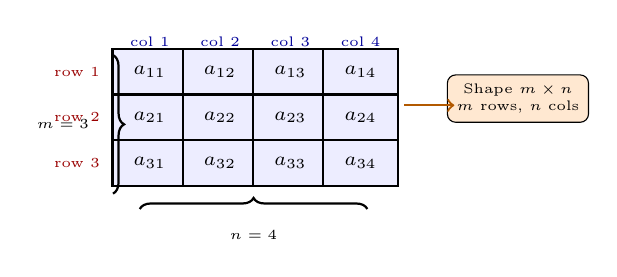
\begin{tikzpicture}[scale=0.85,every node/.style={font=\scriptsize}]
  \foreach \r in {0,...,2} \foreach \c in {0,...,3} {
    \node[draw, thick, minimum width=0.95cm, minimum height=0.58cm, fill=blue!7] at (\c*1.05,\r*-0.68) {$a_{\the\numexpr\r+1\relax\the\numexpr\c+1\relax}$};
  }
  \foreach \c in {0,...,3} \node[font=\tiny,blue!60!black] at (\c*1.05,0.45) {col \the\numexpr\c+1\relax};
  \foreach \r in {0,...,2} \node[font=\tiny,red!60!black,anchor=east] at (-0.6,\r*-0.68) {row \the\numexpr\r+1\relax};
  \draw[decorate,decoration={brace,amplitude=4pt},thick] (-0.55,0.25)--(-0.55,-1.82) node[midway,left=5pt,font=\tiny] {$m=3$};
  \draw[decorate,decoration={brace,amplitude=4pt},thick] (-0.15,-2.05)--(3.25,-2.05) node[midway,below=4pt,font=\tiny] {$n=4$};
  \node[draw,rounded corners=3pt,fill=orange!18,font=\tiny,align=center] at (5.5, -0.4) {Shape $m\times n$\\$m$ rows, $n$ cols};
  \draw[->,thick,orange!70!black] (3.8,-0.5)--(4.55,-0.5);
\end{tikzpicture}
\caption{An $m\times n$ matrix as a table. Row $i$, column $j$ holds $a_{ij}$.}
\label{fig:matrix-anatomy}
\end{figure}

Addition and scalar multiplication are entrywise (same shape required). The zero matrix $0_{m\times n}$ and negatives are as for vectors.

\section{Matrix Multiplication}
\label{sec:mult}
This is the interesting one. Not entrywise --- it composes linear actions.

\begin{definition}[Product]
If $A\in\mathbb{R}^{m\times n}$ and $B\in\mathbb{R}^{n\times p}$, then $C=AB\in\mathbb{R}^{m\times p}$ with
\[
  c_{ij}=\sum_{k=1}^{n} a_{ik}b_{kj}\quad\text{(row $i$ of $A$ dot column $j$ of $B$).}
\]
The inner dimensions must match ($n=n$); the outer give the shape.
\end{definition}

\begin{figure}[h]
\centering
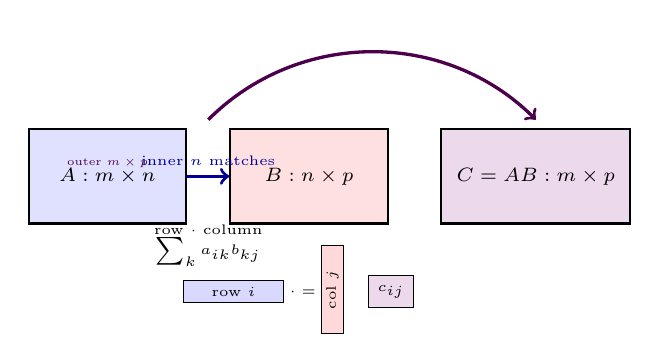
\begin{tikzpicture}[scale=0.80,every node/.style={font=\scriptsize}]
  \node[draw,thick,fill=blue!12,minimum width=2.0cm,minimum height=1.2cm] (A) at (0,0) {$A:m\times n$};
  \node[draw,thick,fill=red!12,minimum width=2.0cm,minimum height=1.2cm] (B) at (3.2,0) {$B:n\times p$};
  \node[draw,thick,fill=violet!15,minimum width=2.4cm,minimum height=1.2cm] (C) at (6.8,0) {$C=AB:m\times p$};
  \draw[->,very thick,blue!60!black] (A)--(B) node[midway,above,font=\tiny] {inner $n$ matches};
  \draw[->,very thick,violet!60!black] (1.6,0.9) to[out=45,in=135] (6.8,0.9) node[midway,above,font=\tiny] {outer $m\times p$};
  \node[font=\tiny,align=center] at (1.6,-1.1) {row $\cdot$ column\\$\sum_k a_{ik}b_{kj}$};
  \begin{scope}[yshift=-2.0cm,xshift=1.2cm]
    \draw[fill=blue!15] (0,0) rectangle (1.6,0.35);
    \draw[fill=red!15] (2.2,-0.5) rectangle (2.55,0.9);
    \node[font=\tiny] at (0.8,0.17) {row $i$};
    \node[font=\tiny,rotate=90] at (2.37,0.2) {col $j$};
    \node[font=\tiny] at (1.9,0.17) {$\cdot=$};
    \node[draw,fill=violet!15,minimum size=0.35cm,font=\tiny] at (3.3,0.17) {$c_{ij}$};
  \end{scope}
\end{tikzpicture}
\caption{Matrix product: inner dimensions agree; entry $c_{ij}$ is the dot product of row $i$ of $A$ with column $j$ of $B$.}
\label{fig:matmul}
\end{figure}

Crucial facts: $AB\neq BA$ in general; $A(BC)=(AB)C$ (associative); $A(B+C)=AB+AC$; there is an identity $I_n$ with $I_nA=A$, $AI_n=A$.

\begin{example}[Composition viewpoint]
If $B:\mathbb{R}^p\to\mathbb{R}^n$ and $A:\mathbb{R}^n\to\mathbb{R}^m$ are linear maps, then $AB$ is the composition ``do $B$, then $A$.'' Order matters --- just as putting on socks then shoes $\neq$ shoes then socks. That is why $AB\neq BA$.
\end{example}

\subsection{Four Ways to See $A\mathbf{x}$}
For $A\in\mathbb{R}^{m\times n}$, $\mathbf{x}\in\mathbb{R}^n$:
\begin{enumerate}[label=(\roman*)]
    \item \textbf{Row dot:} $(A\mathbf{x})_i=\text{row}_i(A)\cdot\mathbf{x}$.
    \item \textbf{Column combination:} $A\mathbf{x}=x_1\mathbf{a}_1+\cdots+x_n\mathbf{a}_n$ where $\mathbf{a}_j$ is column $j$ of $A$. So $A\mathbf{x}$ lives in the span of the columns.
    \item \textbf{Linear map:} $\mathbf{x}\mapsto A\mathbf{x}$ is linear: $A(c\mathbf{x}+d\mathbf{y})=cA\mathbf{x}+dA\mathbf{y}$.
    \item \textbf{Outer sum:} $AB=\sum_{k}\mathbf{a}_k\mathbf{b}_k^T$ (sum of column-times-row rank-one pieces).
\end{enumerate}
View (ii) is the most useful: the columns tell you where the basis lands.

\begin{figure}[h]
\centering
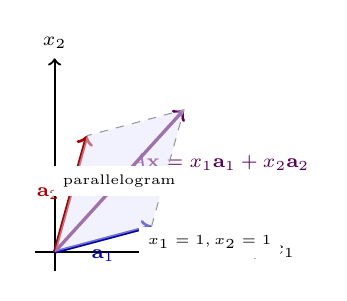
\begin{tikzpicture}[scale=0.82,every node/.style={font=\scriptsize}]
  \draw[->,thick] (-0.3,0)--(3.2,0) node[right] {$x_1$};
  \draw[->,thick] (0,-0.3)--(0,3.0) node[above] {$x_2$};
  \draw[->,very thick,blue!65!black] (0,0)--(1.5,0.4) node[midway,below] {$\mathbf{a}_1$};
  \draw[->,very thick,red!65!black] (0,0)--(0.5,1.8) node[midway,left] {$\mathbf{a}_2$};
  \draw[->,very thick,violet!70!black] (0,0)--(2.0,2.2) node[midway,above right] {$A\mathbf{x}=x_1\mathbf{a}_1+x_2\mathbf{a}_2$};
  \draw[dashed,gray] (1.5,0.4)--(2.0,2.2)--(0.5,1.8);
  \fill[blue!10,opacity=0.5] (0,0)--(1.5,0.4)--(2.0,2.2)--(0.5,1.8)--cycle;
  \node[font=\tiny,fill=white] at (1.0,1.1) {parallelogram};
  \node[font=\tiny,fill=white] at (2.4,0.15) {$x_1=1,x_2=1$};
\end{tikzpicture}
\caption{$A\mathbf{x}$ as a linear combination of the columns $\mathbf{a}_1,\mathbf{a}_2$ of $A$. The set of all $A\mathbf{x}$ is the column span.}
\label{fig:col-combo}
\end{figure}

\section{Transpose and Special Matrices}
\label{sec:transpose}
\begin{definition}[Transpose]
$(A^T)_{ij}=A_{ji}$ --- flip across the diagonal. $(AB)^T=B^TA^T$, $(A^T)^T=A$.
\end{definition}
$A$ is \emph{symmetric} if $A^T=A$ (square, $a_{ij}=a_{ji}$); \emph{diagonal} if $a_{ij}=0$ for $i\neq j$; \emph{upper triangular} if $a_{ij}=0$ for $i>j$; \emph{identity} $I_n=\operatorname{diag}(1,\dots,1)$.

Trace: $\operatorname{tr}(A)=\sum_i a_{ii}$; $\operatorname{tr}(AB)=\operatorname{tr}(BA)$.

\begin{example}[Outer product]
For $\mathbf{u}\in\mathbb{R}^m$, $\mathbf{v}\in\mathbb{R}^n$, the outer product $\mathbf{u}\mathbf{v}^T\in\mathbb{R}^{m\times n}$ has rank one. Inner product $\mathbf{u}^T\mathbf{v}$ is $1\times1$ (a scalar). This distinction matters in ML: $\mathbf{x}\mathbf{x}^T$ is a covariance building block.
\end{example}

\begin{example}[Python --- matrix arithmetic]
\begin{lstlisting}[language=Python]
import numpy as np
A = np.array([[1,2,3],[4,5,6]], dtype=float)  # 2x3
B = np.array([[1,0],[0,1],[1,1]], dtype=float)  # 3x2
C = A @ B            # 2x2 matrix product
print(C)             # [[4,5],[10,11]]
print(A.T.shape)     # (3,2) -- transpose flips shape
# Column view: A @ x = x[0]*col0 + x[1]*col1 + x[2]*col2
x = np.array([1, -1, 2])
print(A @ x, 1*A[:,0] + -1*A[:,1] + 2*A[:,2])
\end{lstlisting}
\end{example}

% ============================================================

% --- Additional depth: Inverses and linear maps ---
\section{Matrix Inverses}
\label{sec:inverses}
$A\in\mathbb{R}^{n\times n}$ is \emph{invertible} (nonsingular) if there exists $A^{-1}$ with $AA^{-1}=A^{-1}A=I_n$. Then $A\mathbf{x}=\mathbf{b}$ has unique solution $\mathbf{x}=A^{-1}\mathbf{b}$, and $A$ represents a bijective linear map. Not all square matrices are invertible: $\begin{bmatrix}1&2\\2&4\end{bmatrix}$ squashes $\mathbb{R}^2$ onto a line.

\begin{theorem}[Invertibility checklist]
For $A\in\mathbb{R}^{n\times n}$, TFAE: (i) $A$ invertible; (ii) $\mathcal{N}(A)=\{\mathbf{0}\}$; (iii) $\mathcal{C}(A)=\mathbb{R}^n$; (iv) $\operatorname{rank}A=n$; (v) $\det A\neq0$ (Ch.~7); (vi) columns (equivalently rows) are independent.
\end{theorem}

$2\times2$ inverse: $\begin{bmatrix}a&b\\c&d\end{bmatrix}^{-1}=\frac1{ad-bc}\begin{bmatrix}d&-b\\-c&a\end{bmatrix}$ when $ad-bc\neq0$. For larger $n$, elimination on $[A\mid I]$ yields $[I\mid A^{-1}]$.

\section{Linear Maps and Matrix Representation}
\label{sec:linmap-detail}
A function $T:\mathbb{R}^n\to\mathbb{R}^m$ is \emph{linear} if $T(c\mathbf{u}+d\mathbf{v})=cT(\mathbf{u})+dT(\mathbf{v})$. Every such $T$ is $\mathbf{x}\mapsto A\mathbf{x}$ for a unique $A$ whose columns are $T(\mathbf{e}_j)$ ($\mathbf{e}_j$ standard basis). Composition $S\circ T$ corresponds to product $BA$.

\begin{example}[Rotation in $\mathbb{R}^2$]
Rotation by $\theta$ counter-clockwise: $R_\theta=\begin{bmatrix}\cos\theta&-\sin\theta\\\sin\theta&\cos\theta\end{bmatrix}$. Then $R_\theta R_\phi=R_{\theta+\phi}$ and $R_\theta^T=R_{-\theta}=R_\theta^{-1}$ (orthogonal matrix).
\end{example}



\begin{remark}[Why $AB\neq BA$ matters in code]
In NumPy, \texttt{A @ B} and \texttt{B @ A} may even have different shapes. Computationally, $(AB)\mathbf{x}=A(B\mathbf{x})$ suggests parenthesising to minimise flops: for $A\in\mathbb{R}^{10\times100}$, $B\in\mathbb{R}^{100\times10}$, $\mathbf{x}\in\mathbb{R}^{10}$, compute $B\mathbf{x}$ first ($100\times10$ by $10$ $\to O(1000)$) then $A(\cdot)$ rather than forming $AB$ ($10\times10$ costs $O(10\cdot100\cdot10)=10^4$). Order and bracketing affect both meaning and cost.
\end{remark}

\begin{example}[Sparse matrices]
Many computing matrices are sparse (mostly zeros): adjacency of a graph, finite differences. Storing only nonzeros and multiplying by iterating over nonzeros saves $O(n^2)$ to $O(\text{nnz})$. \texttt{scipy.sparse} does this; dense \texttt{@} would waste time on zeros.
\end{example}



\begin{example}[Hadamard vs.\ matrix product]
Entrywise (Hadamard) $A\circ B=[a_{ij}b_{ij}]$ is sometimes written $A*B$ in code (e.g.\ NumPy \texttt{A*B} for arrays). It is commutative and $O(mn)$, but it is \emph{not} the matrix product $AB$. Mixing them is a common bug: check whether you need \texttt{A @ B} (composition) or \texttt{A * B} (masking/scaling).
\end{example}

\begin{remark}[Transpose and symmetry in computing]
Storing $A^T$ is often free (stride trick, not a copy) in NumPy; \texttt{A.T} is a view. Symmetry $A^T=A$ halves storage; triangular storage saves half the entries. Numerical libraries exploit this: Cholesky for symmetric positive-definite $A$ is $2\times$ faster than $LU$.
\end{remark}


\section{Chapter Notes}
Matrix multiplication as composition explains non-commutativity and associativity at once. The column picture anticipates column space and rank (Ch.~5) and the $A=LU$ factorisation (Ch.~3). For cost, $m\times n$ times $n\times p$ is $O(mnp)$ naively; Strassen (Ch.~3 notes) does better.

% ============================================================
\section{Exercises}
\label{sec:ch02-exercises}
\begin{enumerate}[label=E2.\arabic*, leftmargin=*, itemsep=0.8em]
\item \textbf{Product by hand.} Let $A=\begin{bmatrix}2&-1&0\\1&3&2\end{bmatrix}$, $B=\begin{bmatrix}1&2\\0&-1\\3&1\end{bmatrix}$. Compute $AB$ and $BA$ (if defined). Verify $(AB)^T=B^TA^T$ numerically.
\item \textbf{Column view.} Write $A=\begin{bmatrix}1&2\\3&4\\5&6\end{bmatrix}$ and $\mathbf{x}=[2,-1]^T$. Compute $A\mathbf{x}$ both as row-dots and as a combination of columns. What is the set $\{A\mathbf{x}:\mathbf{x}\in\mathbb{R}^2\}$ geometrically?
\item \textbf{Algebra.} Prove: if $A,B$ symmetric and $AB=BA$ then $AB$ is symmetric. Give a $2\times2$ counterexample when they do not commute.
\item \textbf{Block multiply.} Let $M=\begin{bmatrix}I&A\\0&I\end{bmatrix}$ where $A$ is $n\times n$. Find $M^2$ and $M^{-1}$ in block form and verify by block multiplication.
\item \textbf{Coding.} Benchmark \texttt{A @ B} for $n\times n$ random matrices ($n=100,500,1000$) with NumPy. Plot time vs.\ $n$ on a log--log scale and estimate the empirical exponent. Why is NumPy far faster than triple loops?
\end{enumerate}
% End of Chapter 2
